\section{Results}\label{sec:Results}

\subsection{Overall model comparison}\label{sec:results-overall}

Table~\ref{tab:main_results} compares the encoder against the TCN baseline on the two primary metrics, root mean squared error (RMSE) and mean absolute error (MAE), averaged over the full forecast horizon and all LOSO folds.

The RMSE for the encoder outperforms the TCN baseline by 10.19\si{\degree}, indicating that the encoder effectively reduces the large-magnitude prediction errors. Furthermore, the encoder achieves a lower MAE, improving upon the baseline by 9.11\si{\degree}. This demonstrates that the encoder's predictions maintain a much tighter average alignment with the true kinematic trajectory of the knee joint.

\begin{table}[htbp]
    \centering
    \caption{Overall LOSO test-set performance averaged over the complete forecast horizon.}
    \label{tab:main_results}
    \resizebox{\columnwidth}{!}{%
    \begin{tabular}{lcc}
        \toprule
        Model & RMSE (\si{\degree}) & MAE (\si{\degree}) \\
        \midrule
        TCN          & 24.50 & 19.24 \\
        Transformer  & \textbf{14.31} & \textbf{10.13} \\
        \bottomrule
    \end{tabular}%
    }
\end{table}

\subsection{Error as a function of forecast horizon}\label{sec:results-horizon}

Figure~\ref{fig:rmse_over_horizon} shows per-step RMSE as a function of position
within the \num{137}-sample forecast window, for the Transformer encoder.

\begin{figure}[htbp]
    \centering
    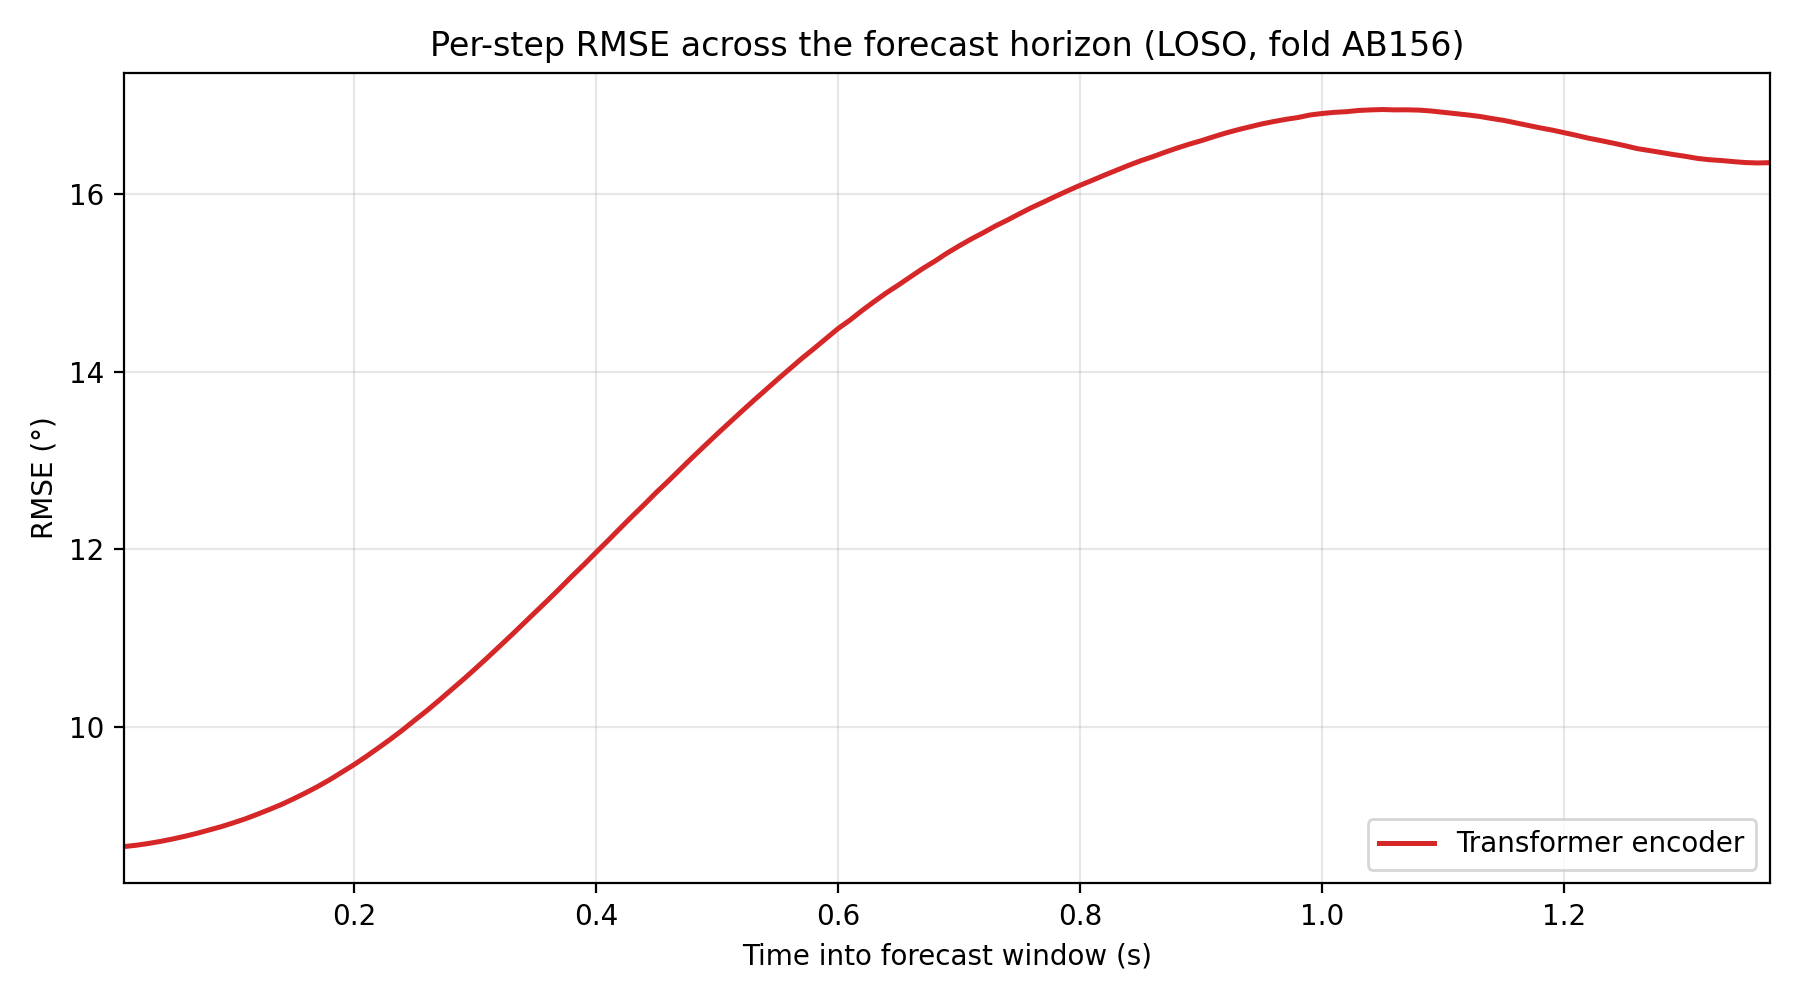
\includegraphics[width=0.85\linewidth]{img/rmse_over_horizon.png}
    \caption{Per-step RMSE across the forecast horizon}
    \label{fig:rmse_over_horizon}
\end{figure}

RMSE rises from \SI{8.65}{\degree} at the first forecast step to a peak of
approximately \SI{16.95}{\degree} around \SI{1.0}{\second}--\SI{1.1}{\second} into
the forecast window, before plateauing and declining slightly to
\SI{16.35}{\degree} by the final step. Error therefore does not grow
monotonically across the full horizon: it increases for roughly the first
three-quarters of the window and then flattens, with the worst-case error
concentrated around the one-second mark rather than at the far end of the
forecast.

\subsection{Error by activity}\label{sec:results-activity}

Figure~\ref{fig:activity_rmse} breaks down RMSE by activity
type. For the encoder error is lowest for ramp ascent/descent (\SI{11.97}{\degree} and
\SI{11.91}{\degree}) and highest for stair ascent (\SI{17.49}{\degree}), with
level walking and stair descent falling in between
(\SI{15.04}{\degree} and \SI{15.18}{\degree}).

\begin{figure}[htbp]
    \centering
    \includegraphics[width=0.7\linewidth]{img/Figure_1.png}
    \caption{RMSE by activity type.}
    \label{fig:activity_rmse}
\end{figure}

For the TCN baseline ranking across activities: lowest for ramp ascent (\SI{22.69}{\degree}),
followed by ramp descent (\SI{23.47}{\degree}), stair ascent
(\SI{25.03}{\degree}), and highest for level walking and stair descent
(\SI{25.09}{\degree} and \SI{25.71}{\degree}, respectively).

\subsection{Ablation dataset split}\label{sec:results-split}

The main results above use the LOSO protocol, in which the held-out test subject
contributes no trials to training and the model must generalize to an entirely
unseen individual. To analyze the cost of this subject-independent generalization
requirement, both models were additionally evaluated under a within-subject split,
in which each subject's own trials are partitioned \SI{70}{\percent}/\SI{10}{\percent}/\SI{20}{\percent}
into train/validation/test respectively and pooled across subjects, so that the training set
contains trials from the same subjects as the test set.

\begin{table}[htbp]
    \centering
    \caption{Test-set RMSE and MAE under the LOSO split versus the within-subject split.}
    \label{tab:split_strategy}
    \resizebox{\columnwidth}{!}{%
    \begin{tabular}{llcc}
        \toprule
        Model & Split strategy & RMSE (\si{\degree}) & MAE (\si{\degree}) \\
        \midrule
        \multirow{2}{*}{TCN}         & LOSO          & 24.50 & 19.24 \\
                                      & Within-subject & 12.30 & 8.73 \\
        \multirow{2}{*}{Transformer} & LOSO          & 14.31 & 10.13\\
                                      & Within-subject & \textbf{7.03} & \textbf{4.32}\\
        \bottomrule
    \end{tabular}%
    }
\end{table}

For the Transformer encoder, mean RMSE lowered from \SI{14.31}{\degree} under the
LOSO split to \SI{7.03}{\degree} under within-subject, confirming that a substantial share of the model's apparent accuracy depends on specific subjects traits

Under the within-subject split, the TCN baseline
achieved a mean RMSE of \SI{12.30}{\degree}
and MAE of \SI{8.73}{\degree}, \SI{12.20}{\degree} and \SI{10.51}{\degree}
lower, respectively, than the LOSO dataset.
However still with this dataset split the encoder holds up agains the TCN baseline

\subsection{Computational footprint}\label{sec:results-compute}

Beyond predictive accuracy, the deployment context motivating this work —
wearable, embedded control of a prosthesis or exoskeleton
(Section~\ref{sec:Materials}) — imposes constraints on model size and
inference latency. Table~\ref{tab:compute_comparison} compares both models on
these dimensions, benchmarked on an Apple M-series GPU (MPS backend) using
\texttt{benchmark\_inference.py}.

\begin{table}[htbp]
    \centering
    \caption{Model size and single-sample inference latency on an Apple
    M-series GPU (MPS backend), measured with \texttt{benchmark\_inference.py}.}
    \label{tab:compute_comparison}
    \resizebox{\columnwidth}{!}{%
    \begin{tabular}{lcc}
        \toprule
        Model & Parameters & Latency @ batch 1 (\si{\milli\second})\\
        \midrule
        TCN          & \num{59081}   & 1.00 \\
        Transformer  & \num{4004785} & 16.9 \\
        \bottomrule
    \end{tabular}%
    }
\end{table}

The Transformer encoder has \num{4004785} parameters and a mean single-sample
inference latency of \SI{16.9}{\milli\second} at batch size 1, scaling to a
throughput of approximately \num{1900} samples/\si{\second} at batch size 64.
TCN has only \num{59081} parameters — roughly \num{68}$\times$ fewer — and a
mean single-sample latency of \SI{1.00}{\milli\second}, scaling to a
throughput of approximately \num{17864} samples/\si{\second} at batch size 64.
TCN is therefore both far smaller and roughly \num{17}$\times$ faster than the
Transformer encoder at batch size 1.
